\chapter{Tail-Anchored Protein Datasets}
\sloppy

\section{Abstract}

\section{Introduction}

\gls{ta} proteins are defined by their single carboxy-terminal~\gls{tms} with a cytosolic facing amino-terminus and are a topologically distinct class of intracellular proteins.
~\gls{ta} proteins are involved in a range of key cellular functions including protein translocation \cite{Osborne2005} and apoptosis \cite{Hockenbery1990}.
Additionally, within the~\gls{ta} class of proteins are a set of vesicle fusion proteins called~\gls{snare} proteins \cite{Ungar2003}, which are contain typically hydrophobic \gls{tmh}s \cite{Kalbfleisch2007}.
There is biomedical interest in~\gls{snare} drug delivery mechanisms.
~\gls{snare}s can fuse liposomes containing various drug payloads into the membrane. %reference needed

The \gls{ta} protein's \gls{tmh} is unusual in that it is both the anchor and the targetting factor for the \gls{er} \cite{Kutay1993}.
Furthermore, the hydrophobicity appears to be a determinate factor in the precise delivery mechanistic route that a~\gls{ta} proteins use for insertion~\cite{Rabu2008, Rabu2009}, for which there is evidence demonstrating that are several mechanisms~\cite{Rabu2009, Johnson2013}(Figure \ref{fig:biogenesis-overview}).
%Alternative mechanisms (Kutay et al., 1995; Nyathi et al., 2013; Chartron et al., 2012)


\begin{figure}[!ht]
\centering
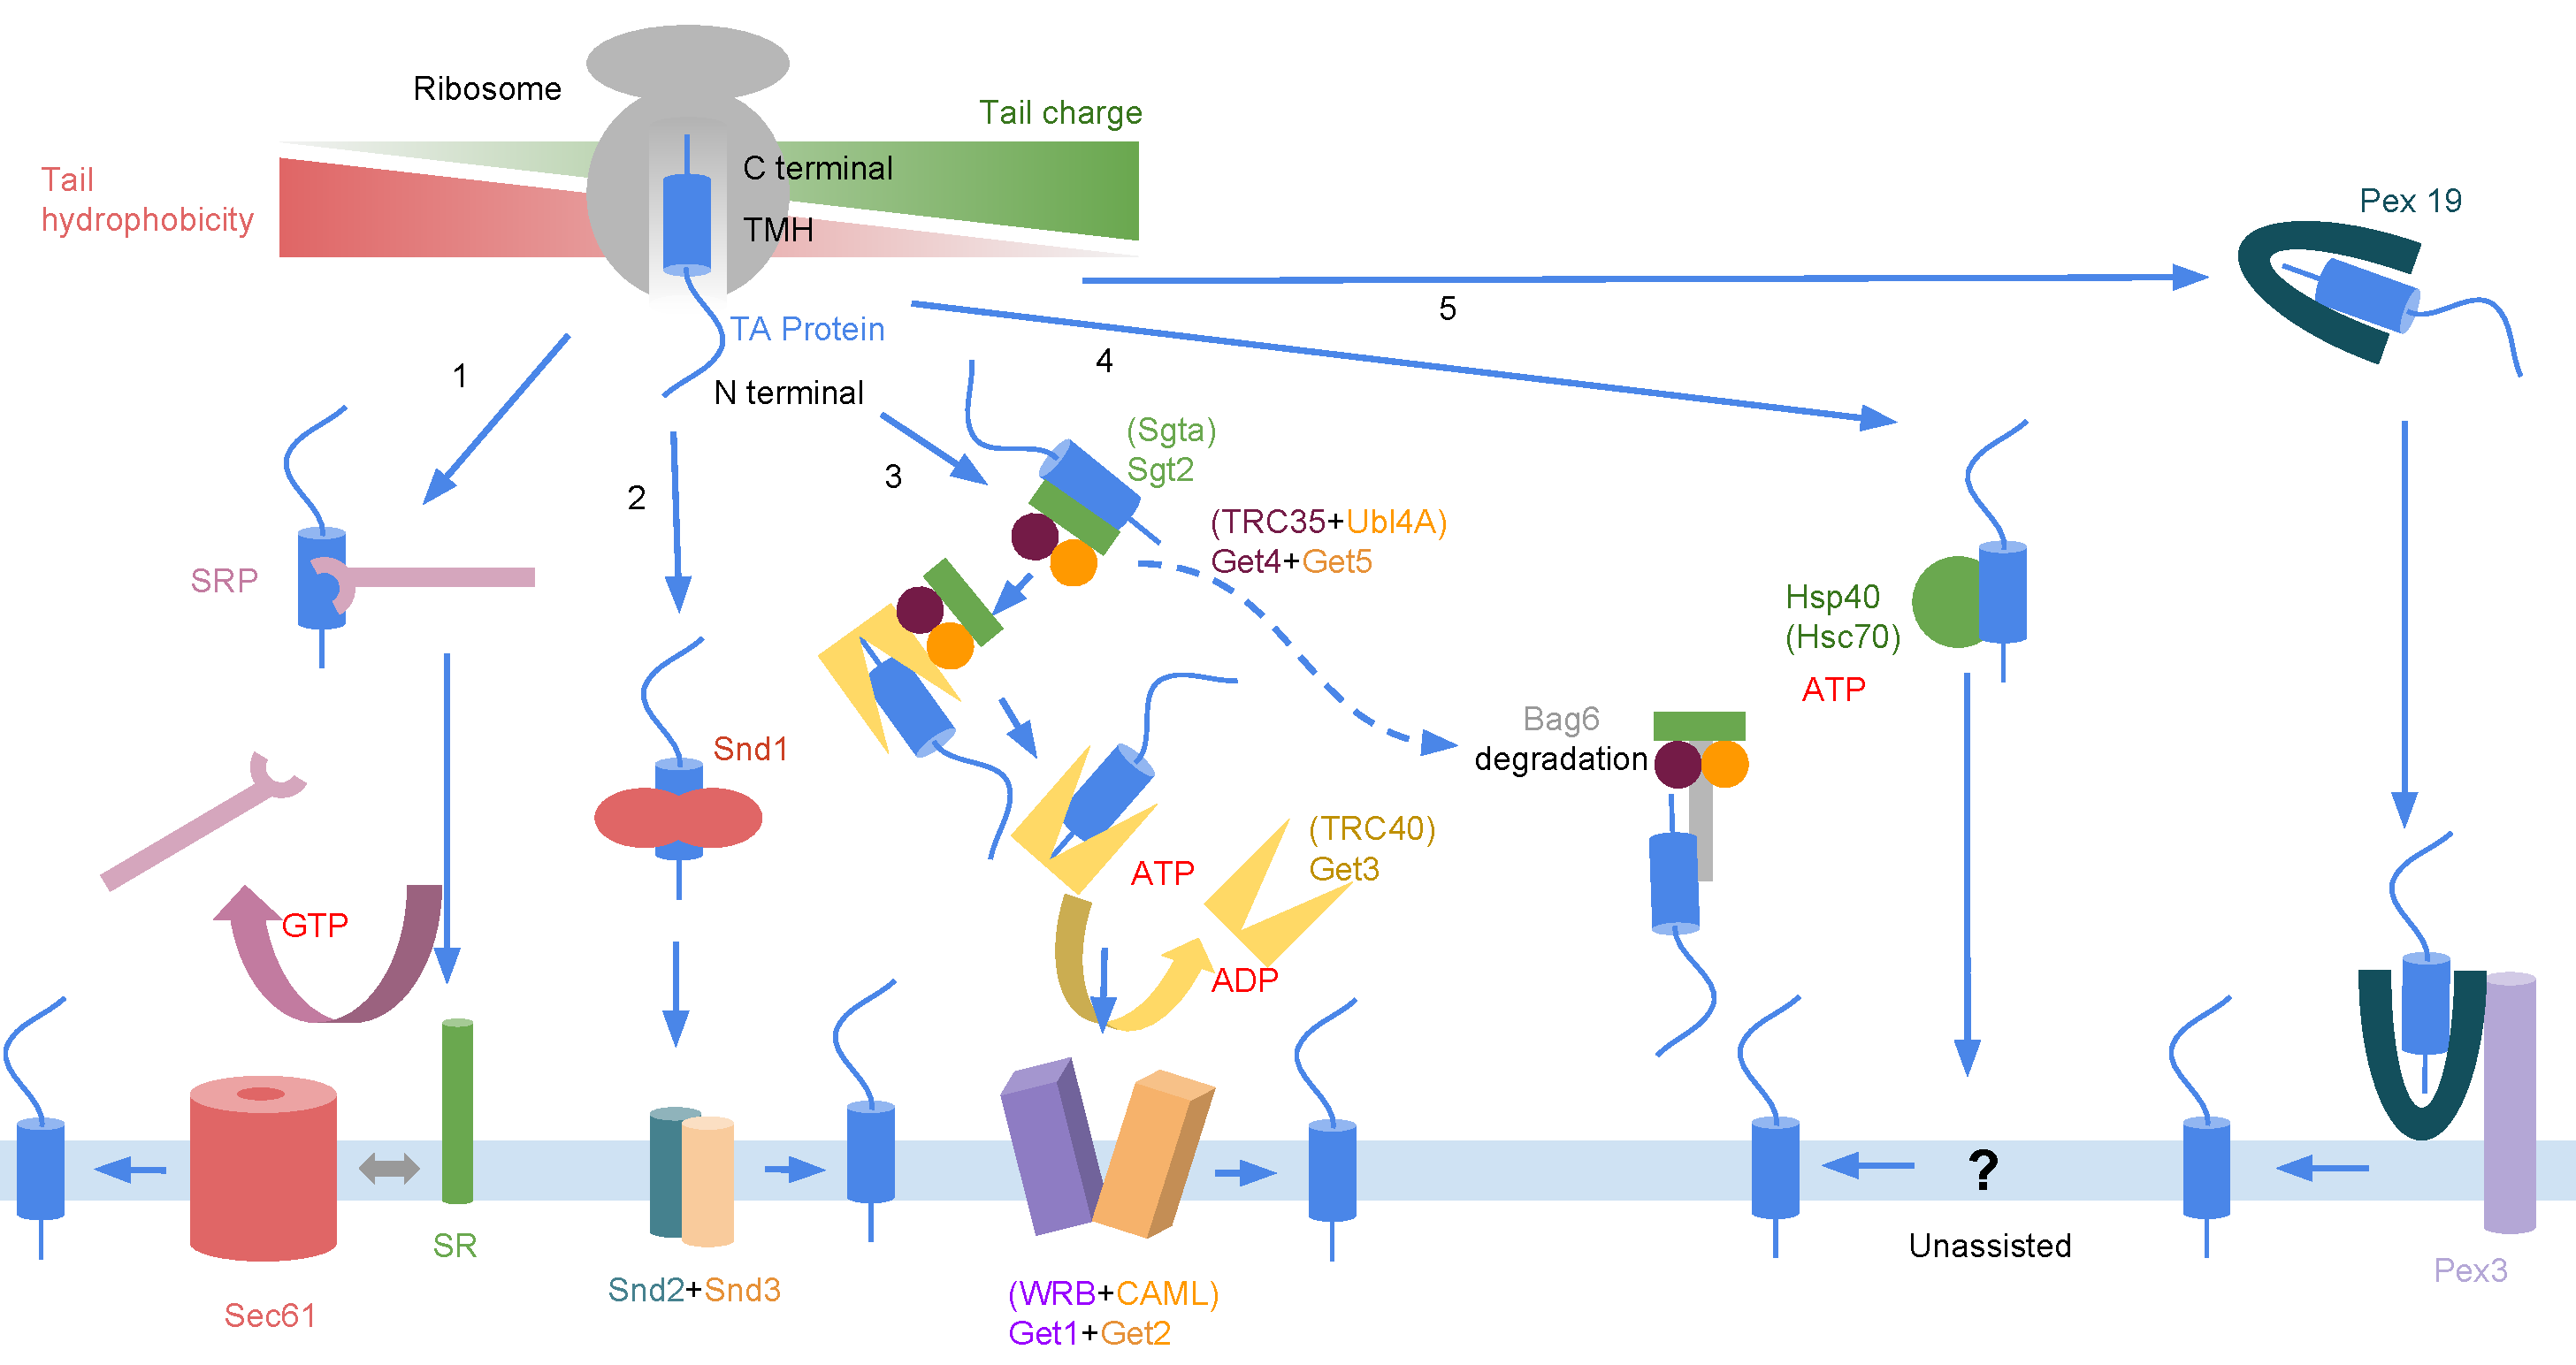
\includegraphics[width=1\textwidth]{TA_chapter/biogenesis-overview}
		\captionof{figure}[An overview of the biogenesis of tail anchored proteins.]{\textbf{An overview of the biogenesis of tail anchored proteins.}
		(1) \gls{srp} and Sec61 of the cotranslational insertion mechanism have been shown to be able to integrate \gls{ta} proteins.
		(2) In yeast a novel mechanism was identified in which Snd1 binds to the folded \gls{ta} protein and delivers it to the membrane bound Snd2 and Snd3 complex.
		(3) The intensively studied Get (yeast) or TRC40 (mammalian) pathway can target either for membrane integration or degradation of the \gls{ta} protein.
		(4) A handful of \gls{ta} proteins with relatively polar \gls{tmh} regions have been observed spontaneously integrating into the membrane using Hsp40 and Hsc70 as chaperones.
		Adapted from Johnson \textit{et al.,} 2013 and Guna \textit{et al.,} 2018.
}

\label{fig:biogenesis-overview}
\end{figure}

\gls{ta} proteins have several pathways for biogenesis in the~\gls{er} membrane.
These mechanisms include the Hsp70/Hsc40 chaperone system~\cite{Rabu2008}, the intensly studied TRC40/Get3 ATP dependent pathway ~\cite{Johnson2013, Chartron2012, Wang2014}, as well as some evidence supporting the use of the co-translational machinery.
\gls{ta} proteins were originally thought to be inserted into the membrane via different machinery than the co-translational machinery, but unexpectedly \gls{srp} was found to be a factor for post-translational targetting confirmed by both cross linking studies \cite{Abell2004} and an \textit{in vitro} pull down experiment \cite{Leznicki2010}.
\gls{srp} would deliver the \gls{ta} protein to the membrane bound \gls{sr} in association with a highly conserved Sec translocon.
Further cross-linking experiments suggested Sec61 is also involved during \gls{ta} protein membrane insertion \cite{Abell2003}.
Previous studies had shown the Sec61 translocon is not necessary for \gls{ta} protein membrane integration by biochemical reconstitution experiments \cite{Kutay1993} and conditional mutants in yeast \cite{Steel2002, Yabal2003}. %What kind of mutants?
This suggests at least one insertion mechanism that is related to the co-translational method of insertion.

A second, possibly redundant, system is also known to be involved in \gls{ta} protein biogenesis and is referred to as the TRC40 (also known as Asna1) pathway in mammals.
A conserved homologue was found in \textit{Saccharomyces cerevisiae}, Get3 \cite{Schuldiner2008}, and in yeast this mechanism is generally referred to as the Get pathway.
Unlike the cotranslational machinery, the post-translational proteins do not couple with the ribosome, so the \gls{ta} protein must be exposed to the cytosolic environment for at least some time \cite{Guna2018}.
At some point after the \gls{ta} protein emerges from the ribosomal exit tunnel, the \gls{ta} protein \gls{tmh} associates with Sgt2.
An \textit{in vitro} assay revealed that Sgt2 associates with Get5  \cite{Wang2010} as part of a dimerised Get4 and Get5 complex (two copies of each)\cite{Chang2010, Chang2012, Chartron2010, Chartron2012}.
At this point Sgt2 either associates with preferential Get3 which targets the \gls{ta} protein for \gls{er} membrane biogenesis, or if there are excess \gls{ta} proteins Sgt2 also associates with Bag6 which targets the \gls{ta} protein for degradation \cite{Shao2017}.
This ``race'' between Bag6 and Get3 ensures a level of quality control within the system.
Assuming the \gls{ta} protein is not targetted for degradation, Get3 associates first with this complex via an interaction with the N-terminal of Get4 \cite{Wang2010}.
A dimerised ADP-bound Get3 \cite{Mateja2009, Hu2009, Bozkurt2009, Suloway2009, Yamagata2009} (TRC40) associates with and shields the C-terminal region of the \gls{ta} protein \cite{Stefanovic2007, Schuldiner2008, Favaloro2008}.
This shielding may be especially important since Get3 is involved in the folding of any nascent \gls{ta} proteins, which would be unviably hydrophobic in the cytosol \cite{Jonikas2009}.
Fluoresence studies revealed that tagged Get3 appears at both the cytosol and the \gls{er} membrane so apparently shuttles the \gls{ta} protein between the transmembrane complex of Get1 and Get 2 (WRB and CAML), that contains cytosolic domains that recieve Get3, and Get4 Get5 Sgt2 complex \cite{Huh2003, Zalisko2017}.
Yet it is an interesting note that a single molecule fluoresence study revealed that the minimum machinery required for \gls{ta} protein insertion from this system is a Get1 and Get2 heterodimer \cite{Zalisko2017}.

Redundancy of the Get/TRC40 pathway and \gls{srp} pathway may be explained in part by a novel \gls{srp} and Get independent pathway.
This pathway utilises the Snd protein pathway and was discovered in yeast \cite{Aviram2016}.
Snd1 binds to the \gls{ta} protein after it exits the ribsosome and delivers it to the Snd2 and Snd3 membrane bound complex which integrate the \gls{ta} protein into the membrane.

In the absence of the Get machinery, Hsp70 and Hsc40 chaperones along with ATP are also sufficient for enough biogenesis of \gls{ta} proteins for viable cell growth \cite{Rabu2008, Rabu2009, Ngosuwan2003, Colombo2009, Kemper2008, Meineke2008, Setoguchi2006}.
Chimeric synaptobrevin, one of the first identified~ \gls{snare} proteins, is capable of spontaneous insertion if the tail anchor domain is replaced by the~\gls{tm} domains belonging to a protein of known spontaneously inserting domains. %citation
Molecular dynamics simulations showed that direct insertion \gls{tmh}s thermodynamically mimics the energies of \gls{tmh}s integrated by the translocon \cite{Ulmschneider2014} so in theory no integration machinery is strictly necessary if the \gls{tmh} can ``correctly'' interact with the membrane interface.
Altering the hydrophobicity, at least in the case of the spontaneously inserting PTP1b, also determinates the localisation of the \gls{ta} protein to either the mitochondrial membrane or the \gls{er} membrane, or rather a more hydrophobic \gls{ta} protein \gls{tmh} is less likely to localise to the mitochondrial membrane \cite{Fueller2015}.


Given a ``choice'', it is speculated that hydrophobicity determines the integration pathway since Sec61$\beta$ has a hydrophobic \gls{tmh} and is targetted via the \gls{srp} pathway, whereas marginally hydrophobic \gls{ta} proteins like cytochrome b5 and PTP1b can spontaneously insert \textit{in vitro} and biologically only rely on Hsp70 and Hsc40.
Broader analysis has shown that hydrophobicity \cite{White1999} stratified by TM tendency score \cite{Zhao2009} can distinguish between the \gls{er} and mitochondrial localised \gls{ta} proteins \cite{Guna2018}.
However, the trememndous diversity and known biogenesis redundancy of these proteins may mean that no single factor applied en masse may be able to distinguish the \gls{tmh} recognition factors and investigation into this area is becoming increasingly complex \cite{Guna2018}.

By regenerating a list of likely \gls{tmh}s \cite{Kalbfleisch2007} and using a manually curated list of \gls{ta} proteins \cite{TheUniProtConsortium2014}, this investigation aims to find relationships between biochemical factors and a disposition to a certain insertion mechanism and terminal localisations.
Here, we also present evidence for a conserved polar strip along the spontaneously inserting \gls{ta} protein \gls{tmh}s, which may be the key to the initial interaction of these \gls{tmh}s with the membrane interface.



\section{Methods}

\subsection{Building a List of Tail-Anchors}
Steps carried out by Kalbfleisch \textit{et al.} published in Traffic 2007 (8: 1687\-1694)~\cite{Kalbfleisch2007}, were recreated using up to date tools.
Whilst their study focused on the human proteome, here we take into account the entire TrEMBL and SwissProt database and then stratify the datasets by the organism at the end of the pipeline.

\subsubsection{SwissProt Tail Anchored Dataset According to Filters}
There were 557012 protein records downloaded from SwissProt via UniProt~\cite{TheUniProtConsortium2014} (Downloaded 24--04--2018).
106149~\gls{tmh}s (\url{TRANSMEM} annotation) were found between 76953 records (\url{annotation:(type:transmem) AND reviewed:no}).
This keyword is contained in a record according to either experimental evidence~\cite{TheUniProtConsortium2014} or a robust meta-analysis of~\gls{tmh} prediction using TMHMM~\cite{Krogh2001}, Memsat~\cite{Jones2007}, Phobius~\cite{Kall2004,Kall2007} and the hydrophobic moment plot method of Eisenberg and co-workers~\cite{Eisenberg1984}.
11141 of those records had only a single~\gls{tmh}.
11110 of those~\gls{tmh}s were within the length thresholds of 16 to 30 residues (None of those had the annotation for splice isoforms according to \url{NON_TER} annotation).
5548 of those had had no~\gls{sp} annotation (\url{SIGNAL}).
4332 of those had annotation (based on \url{TOPO_DOM} annotation) that the N terminal was cytoplasmic.
615 of those had the~\gls{tmh} within 25 residues of the C terminal, the same threshold used by Kalbfleisch and their coworkers~\cite{Kalbfleisch2007}.
Running CD-Hit 4.5.3 on the WebMGA web-server~\cite{Huang2010, Wu2011} at 90\% identical sequence at 90\% coverage thresholds resulted in 443 representative proteins.
This threshold was chosen as a compromise between avoiding over-representation of a certain protein and maintaining a viable sample size.

From this representative list, 46 were Archaeal, 66 were bacterial, and 320 were Eukaryotic and 11 came from dsDNA viruses.
When counting proteomes with greater than 20 records, 49 belonged to the \textit{A. thaliana} proteome, 48 to Mouse, 46 to the human proteome, 24 to \textit{S.cerevisiae}. %19 from RAT!

65 were annotated under the Mitochondrion location (query \url{locations:(location:"Mitochondrion [SL-0173]")}), 157 in the \gls{pm} (query \url{locations:(location:"Cell membrane [SL-0039]")}, 82 in the Golgi (query \url{locations:(location:"Golgi apparatus [SL-0132]")}), and 98 in the \gls{er} (query \url{locations:(location:"Endoplasmic reticulum [SL-0095]"}).

\subsubsection{TrEMBL Tail Anchored Dataset According to Filters}
111425234 records were stored in the TrEMBL database at time of download (Downloaded 25--04--2018).
22107826 of those contained \url{TRANSMEM} annotation (\url{annotation:(type:transmem) AND reviewed:no}).
18053 of these were single-pass proteins.
All of these were within the length restrictions.
17973 of those did not contain a signal sequence when looking for \url{SIGNAL} annotation.
5157 of those contained a cytoplasmically located N terminal according to \url{TOPO_DOM} annotation.
155 records had a~\gls{tmh} within 15 residues of the C terminal residue.
In those record's annotations, no more than 1 appeared in any given species, so they were omitted from the SwissProt list sequence redundancy protocol to avoid representing a well-annotated record with a poorly annotated record.

\subsubsection{UniProt Curated List}
A query for \url{locations:(location:"Single-pass type IV membrane protein [SL-9908]")} was used in UniProt which returned 2460 UniProtKB IDs; 463 SwissProt results and 1997 TrEMBL results.
Running these records through CD-HIT at 90\% redundancy yielded 309 SwissProt records and 808 TrEMBL records~\cite{Huang2010, Wu2011}.
Of those, 987 proteins from 973 records (308 from SwissProt, and 665 from TrEMBL) had the \url{TRANSMEM} annotation indicating a bone fide~\gls{tmh}.
No further filters were applied to this list.
Proteomes represented by more than 20 records include \textit{A. thaliana} (60 records), Humans (38), Mouse (37), and \textit{S. cerevisiae} (31). % and 20 to Rat.

401 were annotated under the Mitochondrion location (query \url{locations:(location:"Mitochondrion [SL-0173]")}) 39 from SwissProt and 362 automatically assigned in TrEMBL.
401 in the \gls{er} (query \url{locations:(location:"Endoplasmic reticulum [SL-0095]"}), 98 from SwissProt and 303 automatically annotated in TrEMBL.
1 TrEMBL record (A0A1E5RT24) in the \gls{er} set contained an ``X'' residue in the C terminal flank and was omitted from the analyses.
Two subcellular location datasets had no automatically ascribed records and only contained manually annotated SwissProt records; 37 in the \gls{pm} (query \url{locations:(location:"Cell membrane [SL-0039]")}, and 82 in the Golgi (query \url{locations:(location:"Golgi apparatus [SL-0132]")}).

\subsubsection{Remapping Previous Dataset}
189 of the 411 proteins from the previous study~\cite{Kalbfleisch2007} were successfully mapped to 222 UniProtKB IDs using the UniProt mapping tools with the RefSeq Protein to UniProtKB option~\cite{TheUniProtConsortium2014}.

\subsection{Calculating Hydrophobicity}
Windowed hydrophobicity was calculated using a window length of 5 residues, and half windows were permitted.
Average hydrophobicity takes the total of the raw amino acid hydrophobicity values and divides them by the number of amino acids in the slice.
Values reported in the results are based on the Kyte \& Doolittle scale~\cite{Kyte1982} which is based on the water\---vapour transfer free energy and the interior-exterior distribution of individual amino acids.
%Hydrophobicity values were also validated by the White and Wimley scale~\cite{White1999}, the Hessa scale~\cite{Hessa2005}, and the Eisenberg scale~\cite{Eisenberg1984}.

\subsection{Calculating Sequence Disorder}

Sequence disorder was calculated from the GlobProt scale~\cite{Linding2003}.
This scale can be used to calculate the tendency within the query protein sequence for order/globularity and disorder.

\subsection{Calculating Sequence Information Entropy}
Information entropy, is essentially an estimate of the linguistic entropy of a string.
In the context of biology, it can be thought of as an estimation of the non-randomness of a sequence.
Sequence complexity can be used to analyse DNA sequences~\cite{Pinho2013, Oliver1993, Troyanskaya2002}, and is a component of the TMSOC z-score which can predict function beyond anchorage of a \gls{tmh}~\cite{Wong2011, Wong2012, Baker2017}.
here we focus on the analysis of the complexity of a sequence in protein sequences.

Broadly speaking, the information theory entropy of a linguistic string can be defined as in equation~\ref{simpleentropy2}, and we treat the protein sequence \gls{tmh} as a string with or without its flanking regions.

\begin{equation} \label{simpleentropy2}
	H(S)=-{\sum_{i=1}^n {p_i\log_s(p_i)}}
\end{equation}

Where H is the entropy of a sequence (S), and $p_i$ is the probability of a character $i$ through each position (n) in S. This allows us to quantify the average relative information density held within a string of information~\cite{Shannon1948}.

\subsection{Statistics}

The null hypothesis of homogeneity of two distributions was examined with the Kolmogorov Smirnov, the Kruskal-Wallis, and the 2-sampled Student's T-test statistical tests.
These tests were all ran through the Python SciPy stat package v0.17 python package~\cite{VanderWalt2011}.
To note, the~\gls{ks} test scrutinises for significant maximal absolute differences between distribution curves; the~\gls{kw} test is after skews between distributions and the student t-test statistical test checks the average difference between distributions.

Since the P‑value is a product of a fraction of test statistics obtained from a permutated set of the samples, it exponentially increases as N increases; the P-value is a strong function of N.
We rely on the Bahadur slope ($B$) as a measure of distance between two distributions~\cite{Bahadur1967, Bahadur1971, Sunyaev1998, Baker2017}. A larger Bahadur slope shows a greater difference between the two distributions.

\begin{equation} \label{eq:bahadur2}
B=\frac{|\ln(P~value)|}{N}
\end{equation}

\subsection{Modelling Cytochrome b5 }
The HHpred webserver was used to query homologues of and model templates for Cytochrome b5 (UniProt accession number P00167) \cite{Soding 2005, Soding 2005a}.
Homologues were queried using three iterations of HHblits25 against the sequence database version uniprot20_2016_02 to generate the query Hidden Markov Model.
The choice of templates was driven by the quality and coverage of the alignments and of the quality of the models that resulted.
A multiple alignment was generated from PDB accession codes 2M33, 2KEO, 3X34, 1MJ4, 1MJ4, 2IBJ covering the globular domain, and PDB accession codes 5NAO, 5DOQ, 5NAM, and 2MMU covering the \gls{tmh}.
Modeller was used to generate a model \cite{Eswar2007}.
The model was confirmed to be of high quality using ProSA (Z-Score: -4.61) \cite{Wiederstein2007}, Ramachandran plot on the RAMPAGE webserver (98\% allowed residues, including all \gls{tmh} residues) \cite{Lovell2003}.
%Verify3D \cite{Luthy1992}, and PROCHECK \cite{Laskowski1993}.

%>P1;UKNP
%sequence:UKNP:1    :A:137  :A::::
%MAEQSDEAVKYYTLEEIQKHNHSK-STWLILHHKVYDLTKFLEEHPGGEEVLREQAGGDATE--NFEDVGHSTDAREMSKTFIIGELHPDDRPKLNKPPETLITTIDSSSSWWTNWVIPAISAVAVALMYRLYMAED*
%>P1;2M33
%structure:2M33:1   :A:104 :A::Oryctolagus cuniculus::
%MAAQSDKDVKYYTLEEIKKHNHSK-STWLILHHKVYDLTKFLEEHPGGEEVLREQAGGDATE--NFEDVGHSTDARELSKTFIIGELHPDDRSKLSKPMETLITTVD------------------------------*
%>P1;2KEO
%structure:2KEO:21  :A:112 :A::Homo sapiens::
%------EKVTLVRIADLENHNNDG-GFWTVIDGKVYDIKDFQTQSLTENSILAQFAGEDPVV--ALEAALQFEDTRESMHAFCVGQYLEPDQEGVTIPDLG------------------------------------*
%>P1;3X34
%structure:3X34:8   :A:92  :A::Sus scrofa:0.76:
%-------AVKYYTLEEIQKHNNSK-STWLILHHKVYDLTKFLEEHPGGEEVLREQAGGDATE--NFEDVGHSTDARELSKTFIIGELHPDDRSKI------------------------------------------*
%>P1;1MJ4
%structure:1MJ4:3   :A:82  :A::Homo sapiens:1.2:
%-------STHIYTKEEVSSHTSPETGIWVTLGSEVFDVTEFVDLHPGGPSKLMLAAGGPLEPFWALYAVHNQSHVRELLAQYKIGEL--------------------------------------------------*
%>P1;2IBJ
%structure:2IBJ:3   :A:88  :A::Musca domestica:1.55:
%-----SEDVKYFTRAEVAKNNTKD-KNWFIIHNNVYDVTAFLNEHPGGEEVLIEQAGKDATE--HFEDVGHSSDAREMMKQYKVGELVAEERSN-------------------------------------------*
%>P1;5NAO
%structure:5NAO:16  :A:34  :A::Homo sapiens::
%-------------------------------------------------------------------------------------------------------------------VLSVLVVSVVAVLVYKFYF---*
%>P1;5DOQ
%structure:5DOQ:6   :C:28  :C::Geobacillus thermodenitrificans (strain NG80-2):3.05:
%------------------------------------------------------------------------------------------------------------------IMYAPMVVVALSVVAAFWVGLKD*
%>P1;5NAM
%structure:5NAM:16  :A:34  :A::Homo sapiens::
%-------------------------------------------------------------------------------------------------------------------VLSVLVVSVVAVLVYKFYF---*
%>P1;2MMU
%structure:2MMU:30  :A:53  :A::Mycobacterium tuberculosis::
%-------------------------------------------------------------------------------------------------------------SVWFVSLFIGLMLIGLIWLMVFQL----*

There are 482 CSI-BLAST hits. 451 of them are unique, including the query.
The calculation is performed on a sample of 150 sequences that represent the list of homologues to the query.

\section{Results}

\subsection{A Comparison Of Up-To-Date Tail-Anchored Protein Datasets}
Here, we use two sources for \gls{ta} protein datasets.
One dataset is based on a previous method~\cite{Kalbfleisch2007} to obtain \gls{ta} datasets and consists of 9296 \gls{tmh} residues (13279 including up to $\pm$5 flanking residues) from 443 SwissProt entries with 90\% redundancy removal.
Another dataset contains the UniProt curated set of Type IV membrane proteins again with 90\% redundancy removal.
This dataset contains 21119 \gls{tmh} residues (28791 including up to $\pm$5 flanking residues) from 987 UniProt protein records.

% Venn diagram
\begin{figure}[!ht]
\centering
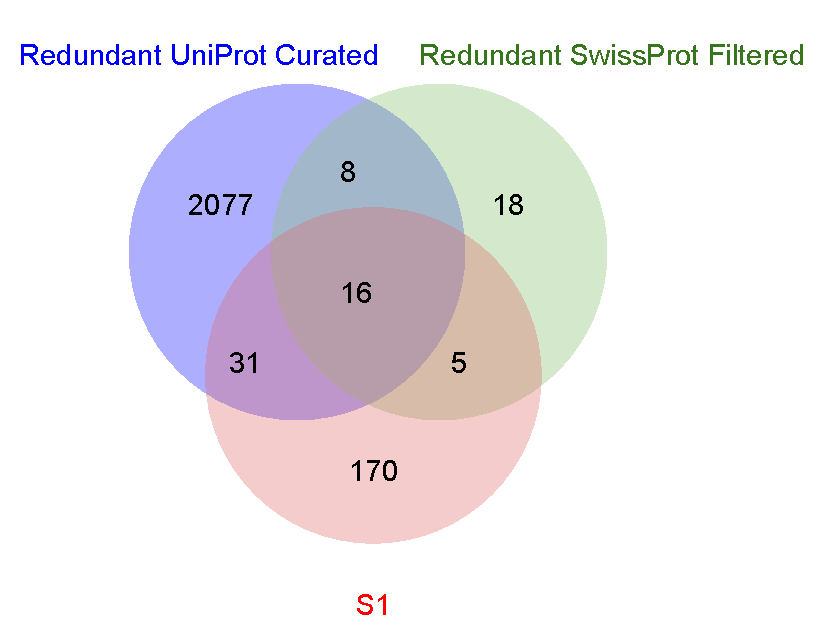
\includegraphics[width=0.5\textwidth]{TA_chapter/database-overlap}
		\captionof{figure}[A Venn diagram showing tail anchored protein UniProt ids present in each of the datasets as well as those present in multiple datasets.]{\textbf{A Venn diagram showing tail anchored protein UniProt ids present in each of the datasets as well as those present in multiple datasets.}
The number of ids present in redundant versions of
i) the supplementary materials table of a previous study predicting the complete set of human tail anchored proteins denote by S1~\cite{Kalbfleisch2007},
ii) the SwissProt dataset filtered according to typical~\gls{ta} features limited to the human proteome~\cite{TheUniProtConsortium2014}, and
iii) The UniProt curated list of~\gls{ta} proteins~\cite{TheUniProtConsortium2014}.
Note that to avoid losing IDs to redundancy reduction this diagram was generated without the use of CD-HIT~\cite{Huang2010, Wu2011}, which is applied in later statistical analysis.}

\label{fig:tadatasetoverlap}
\end{figure}

In order to get an understanding of the consistency of the datasets, before removing redundant proteins, we compared these two datasets to a dataset remapped set of proteins from a previous 2007 method~\cite{Kalbfleisch2007}.
The S1 dataset was built with an aim to gather \gls{ta} proteins in the human genome from the NCBI.
Note that these numbers are not absolutely certain.
The greatest source of uncertainty here is that the original S1 list includes 411 records, however only 222 of these were successfully mapped to the UniProt dataset.
This figure is closer to the 202 proteins from the original S1 list that excluded proteins that were either hypothetical or splice isoforms.
That being said, this mapping step prevents us from directly comparing the entire original S1 dataset.
We compared the up-to-date datasets to S1 to see how many records are shared, how many are now obsolete, and how many are unique.

Figure~\ref{fig:tadatasetoverlap} shows that S1 has 175 record ids of 222 records (78.8\%) which do not share overlap the up-to-date manually curated UniProt dataset~\cite{TheUniProtConsortium2014}.
Of the 166 unique records of that S1 dataset, 92 records do have location annotation in UniProt which our scripts use for topological determination, leaving 74 records without location annotation.
This leaves 92 of the 222 S1 (41.4\%) records that originally fitted criteria that no longer fit those same criteria.
If we exclude those lacking suitable annotation i.e ids from S1 that are found in either SwissProt with the filters (9), the curated UniProt list (14), or both (33), compared to the 92 that have annotation contradicting the original predictions, 37.8\% of the ids overlap.

Equivalent criteria were applied to the entire SwissProt database and then restricted to the human proteome dataset.
43 of these 77 records (55.8\%) are in the curated UniProt~\gls{ta}  dataset leaving 34 records that meet the criteria out of the manually curated set (44.2\%of the filtered SwissProt dataset).
42 of the 77 (54.5\%) records from SwissProt filtered human dataset can be found in the original S1 list.
A further consideration is that, before limiting the dataset to human and after removing redundant proteins, this method picked up  46 archaeal and 66 bacterial records.

The same method applied to an up-to-date dataset overlaps more with a manually curated dataset.
There is also a large degree of what we now believe to be mistakes that occurred in the older prediction tools and datasets, even when using similar methods.
As a trend, this shows that up-to-date datasets improve the reliability of this automated predicted method.
These automated criteria still do not fully align with the manually curated list.
Only 973 of a non-redundant (90\% CD-HIT threshold \cite{Huang2010, Wu2011}) set of those 2460 proteins of the UniProt manually curated set contained annotation for the transmembrane boundary residues.
Ultimately, this points to the idea that datasets are a moving target as they are constantly updated with more accurate and reliable tools.

\subsection{It Is Difficult To Observe Hydrophobic Variation Of TA Protein TMHs From Different Species}

In single-pass proteins of eukaryotic species there are typically various adaptations of the \gls{tmh} to adhere to the membrane constraints of the specific membrane.
For single-pass proteins, previous studies have observed differences in terms of \gls{tmh} hydrophobicity between yeast and human \gls{tmp}s~\cite{Sharpe2010}, or in cress, yeast, bacteria, and human datasets~\cite{Baker2017}.
We would expect to see a similar trend between the \gls{tmh}s of \gls{ta} proteins from different species.
However, when assuming a zero-difference hypothesis, in these \gls{tmh} \gls{ta} protein datasets we cannot observe any species-level differences between the datasets at this sample size for \gls{tmh} hydrophobicity.

% Average lines for figure, table for stats
When comparing the average Kyte \& Doolittle~\cite{Kyte1982} hydrophobicity values for the~\gls{tmh}s from humans and mice, \textit{A. thaliana}, and  \textit{S. cerevisiae}, we can see little difference between the mean values.
All of the mean values lie between 2.3-2.6 when we only consider the \gls{tmh} and at 1.3-1.6 when considering residues in close proximity to the~\gls{tmh} ($\pm$5 residues) (Figure~\ref{fig:average_species_hydrophobicity_ta}).

\begin{figure}[!ht]
\centering
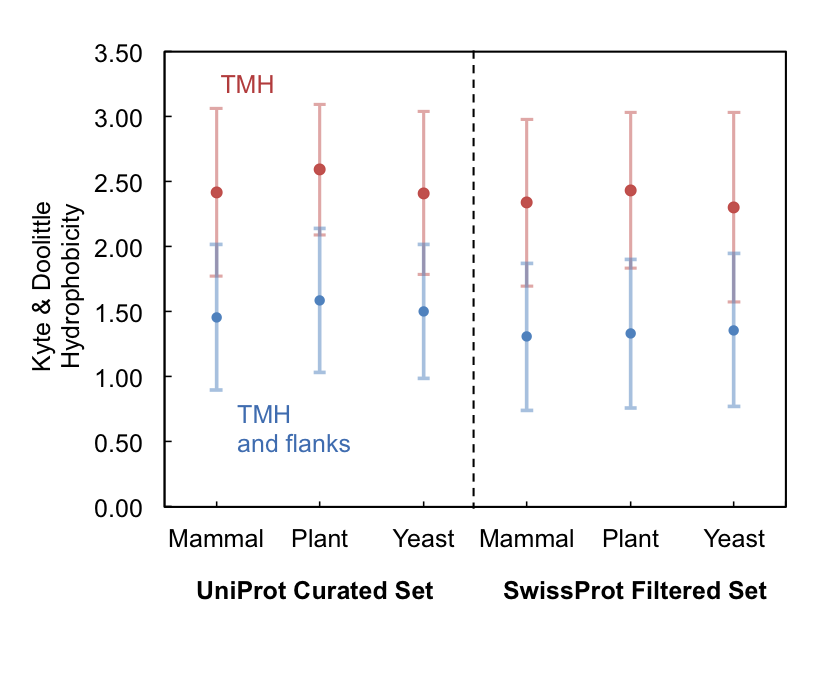
\includegraphics[width=1\textwidth]{TA_chapter/species-hydrophobicity}
\captionof{figure}[Average values of species datasets from UniProt manually curated set and SwissProt automatically filtered dataset.]
{\textbf{Average values of species datasets from UniProt manually curated set and SwissProt automatically filtered dataset.}

The average hydrophobicity values from the Kyte \& Doolittle scale~\cite{Kyte1982}.for both the \gls{tmh} and the \gls{tmh}$\pm$5 residues.
%and the GlobProt scale~\cite{Linding2003}
Values are shown for both the UniProt manually curated set and the SwissProt filtered set. In the UniProt manually curated set we compare the mammalian set of \gls{ta} proteins (Human N=38 and Mouse N=37) to \textit{A. thaliana} (N=60) representing plants and \textit{S. cerevisiae} (N=31) representing yeasts. For the SwissProt filtered set we compare the mammalian set of \gls{ta} proteins (Human N=46 and Mouse N=48) to \textit{A. thaliana} (N=49) representing plants  and  \textit{S. cerevisiae} (N=24) representing yeasts.
Error bars are shown at $\pm 1 \sigma$ from the mean of the respective dataset.
}

\label{fig:average_species_hydrophobicity_ta}
\end{figure}

Indeed, we see no strong observable statistical differences in hydrophobicity ($P>3.35E-1$ in the SwissProt automatically filtered list Table \ref{table:speciestableswissprotstats}, and $P>8.30E-2$ in the UniProt curated list Table \ref{table:speciestableuniprotstats}).
There are also no consistent trends among the absolute Bahadur slopes; no datasets are greatly different from any other.

\begin{table}[htbp]
\centering
\captionof{table}[Hydrophobicity statistical comparisons between mouse and human, yeast, and plants in the SwissProt Filtered Dataset.]
{\textbf{Hydrophobicity statistical comparisons between mouse and human, yeast, and plants in the SwissProt Filtered Dataset.}
Here, we compare a mammalian set of \gls{ta} proteins (Human N=46 and Mouse N=48) to \textit{A. thaliana} (N=49) representing plants  and  \textit{S. cerevisiae} (N=24) representing yeasts.
The hydrophobicity was predicted as the mean average of the values of the sequences of the \gls{tmh}, as well another group including up to $\pm$5 flanking residues, since predicting the boundary of \gls{tmh}s is difficult, according to the Kyte \& Doolittle hydrophobicity scale~\cite{Kyte1982}.
% Disorder was calculated in the same way using the GlobProt scale \cite{Linding2003}.
The Test column refers to the statistical score obtained from the test; H statistic for the Kruskal Wallis, the KS statistic for the Kolmogorov Smirnov test, and the t-statistic for the T-test.
$P$ is the P-value of that statistical score.
$B$ refers to the Bahadur slope, an interpretation of the P-value that accounts for the sample size powering the test~\cite{Bahadur1967, Bahadur1971}.}
\tiny
	% Table generated by Excel2LaTeX from sheet 'SwissProt filtered species'

    \begin{tabular}{clrrrrrrrrr}
          &       & \multicolumn{3}{c}{Mammal and Plant} & \multicolumn{3}{c}{Mammal and Yeast} & \multicolumn{3}{c}{Plant and Yeast} \\
          &       & \multicolumn{1}{l}{Test} & \multicolumn{1}{l}{$P$} & \multicolumn{1}{l}{$B$} & \multicolumn{1}{l}{Test} & \multicolumn{1}{l}{$P$} & \multicolumn{1}{l}{$B$} & \multicolumn{1}{l}{Test} & \multicolumn{1}{l}{$P$} & \multicolumn{1}{l}{$B$} \\
    \multirow{3}[0]{*}{TMH } &  Kruskal-Wallis & 0.93  & 3.35E-1 & 7.64E-3 & 0.10  & 7.56E-1 & 2.37E-3 & 0.84  & 3.60E-1 & 1.40E-2 \\
          &  Kolmogorov-Smirnov & 0.13  & 6.36E-1 & 3.17E-3 & 0.12  & 9.24E-1 & 6.69E-4 & 0.19  & 5.28E-1 & 8.76E-3 \\
          &  Student's T-test & -0.86 & 3.90E-1 & 6.58E-3 & 0.21  & 8.31E-1 & 1.57E-3 & 0.79  & 4.33E-1 & 1.15E-2 \\
    \multirow{3}[0]{*}{TMH and flanks } &  Kruskal-Wallis & 0.04  & 8.52E-1 & 1.12E-3 & 0.12  & 7.28E-1 & 2.69E-3 & 0.04  & 8.33E-1 & 2.51E-3 \\
          &  Kolmogorov-Smirnov & 0.11  & 7.72E-1 & 1.81E-3 & 0.13  & 8.79E-1 & 1.09E-3 & 0.11  & 9.80E-1 & 2.81E-4 \\
          &  Student's T-test & -0.22 & 8.23E-1 & 1.37E-3 & -0.38 & 7.04E-1 & 2.97E-3 & -0.19 & 8.50E-1 & 2.22E-3 \\
    \end{tabular}%
				\label{table:speciestableswissprotstats}

\end{table}%

\begin{table}[htbp]
\centering
\captionof{table}[Hydrophobicity statistical comparisons between mouse and human, yeast, and plants in the UniProt Curated Dataset.]
{\textbf{Hydrophobicity statistical comparisons between mouse and human, yeast, and plants in the UniProt Curated Dataset.}
Here, we compare a mammalian set of \gls{ta} proteins (Human N=38 and Mouse N=37) to \textit{A. thaliana} (N=60) representing plants  and  \textit{S. cerevisiae} (N=31) representing yeasts.
The hydrophobicity was predicted as the mean average of the values of the sequences of the \gls{tmh}, as well another group including up to $\pm$5 flanking residues, since predicting the boundary of \gls{tmh}s is difficult, according to the Kyte \& Doolittle hydrophobicity scale~\cite{Kyte1982}.
%Disorder was calculated in the same way using the GlobProt scale \cite{Linding2003}.
The Test column refers to the statistical score obtained from the test; H statistic for the Kruskal Wallis, the KS statistic for the Kolmogorov Smirnov test, and the t-statistic for the T-test.
$P$ is the P-value of that statistical score.
$B$ refers to the Bahadur slope, an interpretation of the P-value that accounts for the sample size powering the test~\cite{Bahadur1967, Bahadur1971}.}
	\tiny
	% Table generated by Excel2LaTeX from sheet 'SwissProt filtered species'

    \begin{tabular}{clrrrrrrrrr}
	          &       & \multicolumn{3}{c}{Mammal and Plant} & \multicolumn{3}{c}{Mammal and Yeast} & \multicolumn{3}{c}{Plant and Yeast} \\
	          &       & \multicolumn{1}{l}{Test} & \multicolumn{1}{l}{$P$} & \multicolumn{1}{l}{$B$} & \multicolumn{1}{l}{Test} & \multicolumn{1}{l}{$P$} & \multicolumn{1}{l}{$B$} & \multicolumn{1}{l}{Test} & \multicolumn{1}{l}{$P$} & \multicolumn{1}{l}{$B$} \\
	    \multirow{3}[0]{*}{TMH } &  Kruskal-Wallis & 2.15  & 1.42E-1 & 1.45E-2 & 0.22  & 6.39E-1 & 4.22E-3 & 2.30  & 1.30E-1 & 2.25E-2 \\
	          &  Kolmogorov-Smirnov & 0.17  & 2.86E-1 & 9.27E-3 & 0.15  & 6.32E-1 & 4.34E-3 & 0.24  & 1.69E-1 & 1.95E-2 \\
	          &  Student's T-test & -1.71 & 8.96E-2 & 1.79E-2 & 0.04  & 9.70E-1 & 2.86E-4 & 1.47  & 1.46E-1 & 2.11E-2 \\
	    \multirow{3}[0]{*}{TMH and flanks } &  Kruskal-Wallis & 2.17  & 1.41E-1 & 1.45E-2 & 0.14  & 7.13E-1 & 3.19E-3 & 0.59  & 4.41E-1 & 9.00E-3 \\
	          &  Kolmogorov-Smirnov & 0.21  & 8.30E-2 & 1.84E-2 & 0.10  & 9.62E-1 & 3.62E-4 & 0.14  & 8.00E-1 & 2.45E-3 \\
	          &  Student's T-test & -1.33 & 1.86E-1 & 1.25E-2 & -0.39 & 7.00E-1 & 3.36E-3 & 0.69  & 4.90E-1 & 7.83E-3 \\
	    \end{tabular}%
					\label{table:speciestableuniprotstats}
	\end{table}%

Here, we are dealing with datasets at least an order of magnitude smaller than those broad studies \cite{Sharpe2010, Baker2017} which could explain the absence of the effect.
However this only goes to show that if there is an effect in \gls{ta} proteins, it is indeed weak between species.


\subsection{There Are Biochemical Differences Between Tail-Anchored TMHs From Different Organelles}
% Average lines for figure, table for stats

As in the case of species, \gls{tmh}s with different subcellular localisations on average  have different hydrophobicity.
%Need mitochondria reference, and numbers for the UniER etc.
These hydrophobic differences have already been observed in the mitochondria localised \gls{ta} protein \gls{tmh}.
Here we consider the \gls{ta} proteins at certain locations within the cell ignoring species, and we see clear differences in the biochemistry of the \gls{tmh}.
In the UniProt manually curated dataset, the Kyte \& Doolittle hydrophobicity scores rage from 1.7 in mitochondria to 2.7 in the \gls{pm} (Figure \ref{fig:average_organelle_factors_ta}A).

\begin{figure}[!ht]
\centering
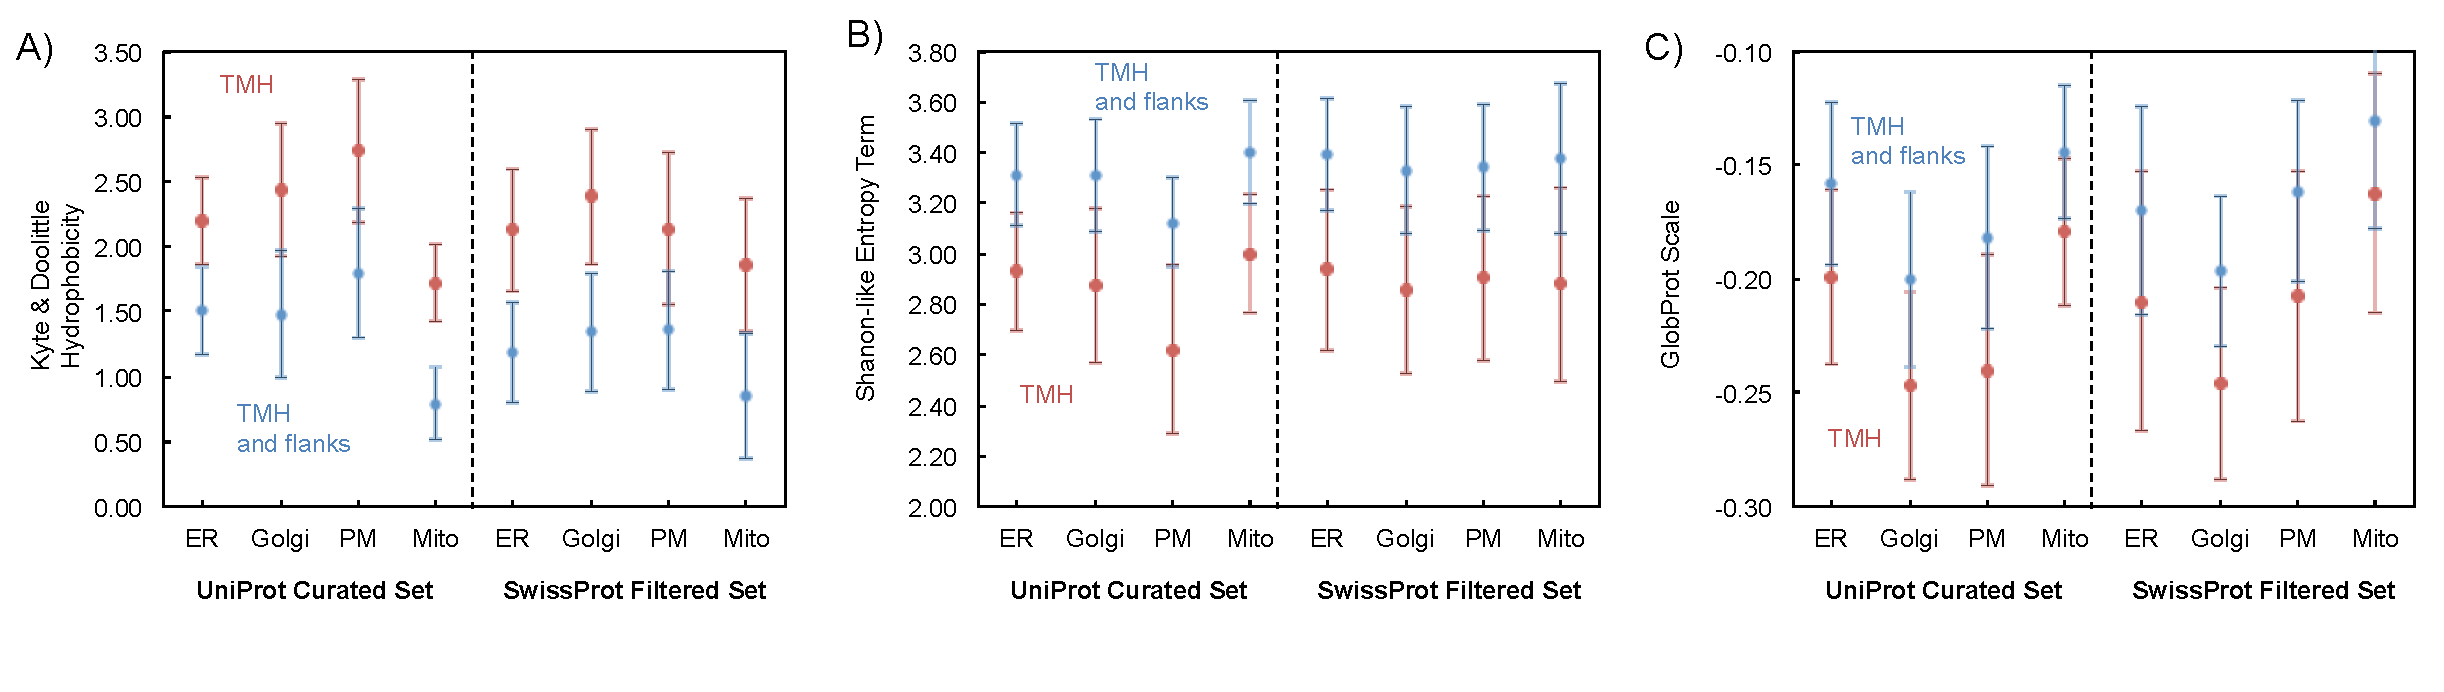
\includegraphics[width=1\textwidth]{TA_chapter/organelle-averages}
\captionof{figure}[Average sequence-based biochemical values of organelle datasets from UniProt manually curated set and SwissProt automatically filtered dataset.]
{\textbf{Average sequence-based biochemical values of organelle datasets from UniProt manually curated set and SwissProt automatically filtered dataset.}

A) The average hydrophobicity values from the Kyte \& Doolittle scale~\cite{Kyte1982}, B) the average information entropy~\cite{Shannon1948} (see methods) and C) the GlobProt scale~\cite{Linding2003} for both the \gls{tmh} and the \gls{tmh}$\pm$5 residues.
Values are shown for both the UniProt manually curated set and the SwissProt filtered set.
In the UniProt manually curated set we compare \gls{ta} proteins from the~\gls{er} (N=400) to the Golgi (N=82), the~\gls{pm} (N=37), and the mitochondria (N=401).
For the SwissProt filtered set we compare \gls{ta} proteins from the~\gls{er} (N=98) to the Golgi (N=82), the~\gls{pm} (N=157), and the mitochondria (N=65).
Error bars are shown at $\pm 1 \sigma$ from the mean of the respective dataset.
}

\label{fig:average_organelle_factors_ta}
\end{figure}




\begin{table}[htbp]
\centering
\captionof{table}[Statistical comparisons between TMH sequences from organelles in the UniProt Curated Dataset.]
{\textbf{Statistical comparisons between TMH sequences from organelles in the UniProt Curated Dataset.}
Here, we compare a organelle subsets from the UniProt curated dataset of \gls{ta} proteins.
We compare \gls{er} (N=400) to Golgi (N=82), \gls{pm} (N=37), and the mitochondria (N=401).
The hydrophobicity was predicted as the mean average of the values of the sequences of the \gls{tmh}, as well another group including up to $\pm$5 flanking residues, since predicting the boundary of \gls{tmh}s is difficult, according to the Kyte \& Doolittle hydrophobicity scale~\cite{Kyte1982}.
Disorder was calculated in the same way using the GlobProt scale \cite{Linding2003}.
The linguistic information entropy was calculated according to the methods section~\cite{Shannon1948}.
The Test column refers to the statistical score obtained from the test; H statistic for the Kruskal Wallis (KW), the KS statistic for the Kolmogorov Smirnov test (KS), and the t-statistic for the student's T-test (T-test).
$P$ is the P-value of that statistical score.
$B$ refers to the Bahadur slope, an interpretation of the P-value that accounts for the sample size powering the test~\cite{Bahadur1967, Bahadur1971}.}
	\tiny

	\begin{tabular}{clrrrrrrrrr}
							&       & \multicolumn{3}{c}{ER and Golgi} & \multicolumn{3}{c}{ER and PM} & \multicolumn{3}{c}{ER and mitochondria} \\
							&       & \multicolumn{1}{l}{Test} & \multicolumn{1}{l}{$P$} & \multicolumn{1}{l}{$B$} & \multicolumn{1}{l}{Test} & \multicolumn{1}{l}{$P$} & \multicolumn{1}{l}{$B$} & \multicolumn{1}{l}{Test} & \multicolumn{1}{l}{$P$} & \multicolumn{1}{l}{$B$} \\
	\midrule
	\multirow{3}[0]{*}{TMH Hydrophobicity} &  KW & 15.84 & 6.89E-5 & 1.93E-2 & 32.82 & 1.01E-8 & 4.17E-2 & 344.94 & 5.36E-77 & 2.15E-1 \\
							&  KS & 0.30  & 2.79E-6 & 2.58E-2 & 0.54  & 2.04E-9 & 4.54E-2 & 0.64  & 3.71E-74 & 2.07E-1 \\
							&  T-test & -5.45 & 7.91E-8 & 3.30E-2 & -8.64 & 1.02E-16 & 8.35E-2 & 21.65 & 1.90E-82 & 2.31E-1 \\
	\midrule
	\multirow{3}[0]{*}{... including flanks} &  KW & 0.95  & 3.30E-1 & 2.24E-3 & 15.29 & 9.22E-5 & 2.11E-2 & 463.33 & 9.05E-103 & 2.88E-1 \\
							&  KS & 0.17  & 1.79E-2 & 8.11E-3 & 0.47  & 3.90E-7 & 3.35E-2 & 0.80  & 1.03E-116 & 3.28E-1 \\
							&  T-test & 0.52  & 6.02E-1 & 1.02E-3 & -4.72 & 3.24E-6 & 2.87E-2 & 32.76 & 1.02E-150 & 4.24E-1 \\
	\midrule
	\multirow{3}[0]{*}{TMH Disorder} &  KW & 79.40 & 5.08E-19 & 8.49E-2 & 24.33 & 8.12E-7 & 3.18E-2 & 60.00 & 9.46E-15 & 3.96E-2 \\
							&  KS & 0.48  & 5.56E-16 & 7.08E-2 & 0.49  & 8.84E-8 & 3.68E-2 & 0.26  & 3.78E-12 & 3.23E-2 \\
							&  T-test & 10.62 & 7.27E-24 & 1.07E-1 & 6.03  & 3.43E-9 & 4.42E-2 & -7.98 & 4.81E-15 & 4.05E-2 \\
	\midrule
	\multirow{3}[0]{*}{... including flanks} &  KW & 74.45 & 6.22E-18 & 7.99E-2 & 13.54 & 2.33E-4 & 1.90E-2 & 33.76 & 6.23E-9 & 2.32E-2 \\
							&  KS & 0.46  & 1.58E-14 & 6.41E-2 & 0.37  & 1.42E-4 & 2.01E-2 & 0.22  & 3.02E-9 & 2.41E-2 \\
							&  T-test & 9.93  & 2.52E-21 & 9.56E-2 & 3.78  & 1.78E-4 & 1.96E-2 & -5.96 & 3.77E-9 & 2.38E-2 \\
	\midrule
	\multirow{3}[0]{*}{TMH entropy} &  KW & 1.33  & 2.49E-1 & 2.80E-3 & 31.76 & 1.75E-8 & 4.05E-2 & 22.64 & 1.95E-6 & 1.61E-2 \\
							&  KS & 0.20  & 3.86E-3 & 1.12E-2 & 0.42  & 6.23E-6 & 2.72E-2 & 0.18  & 1.46E-6 & 1.65E-2 \\
							&  T-test & 1.97  & 4.97E-2 & 6.05E-3 & 7.37  & 8.47E-13 & 6.30E-2 & -4.24 & 2.54E-5 & 1.30E-2 \\
	\midrule
	\multirow{3}[0]{*}{... including flanks} &  KW & 0.16  & 6.93E-1 & 7.39E-4 & 27.12 & 1.91E-7 & 3.51E-2 & 42.77 & 6.15E-11 & 2.88E-2 \\
							&  KS & 0.16  & 3.15E-2 & 6.97E-3 & 0.46  & 5.92E-7 & 3.25E-2 & 0.24  & 1.20E-10 & 2.80E-2 \\
							&  T-test & 0.10  & 9.21E-1 & 1.66E-4 & 5.55  & 4.97E-8 & 3.81E-2 & -6.14 & 1.26E-9 & 2.51E-2 \\
	\end{tabular}%
					\label{table:organellesuniprotstats}
	\end{table}%

In the UniProt curated list, there are clear hydrophobic differences between all the \gls{tmh}s ($P<6.89E-5$) which as a trend becomes less clear when considering the \gls{tmh}$\pm$5 flanking residues except for mitochondria which increases in significance when considering the flanks also (Table~\ref{table:organellesuniprotstats}).
The \gls{er} and mitochondrial tests are very significant ($P<3.71E-74$).
Consistently the Bahadur slope is at least an order of magnitude greater in the \gls{er} and mitochondrial comparison than for the other considerations, so these differences cannot be accounted for by the larger sample size.

In terms of information entropy, there is a marked decrease in entropy in the \gls{pm} subset (mean entropy = 3.12 in the \gls{tmh}, 2.6 including $\pm$5 flanking residues) from the UniProt curated dataset compared to the other organelle datasets (entropy $>$ 3.3 and $>$ 2.8 including the flanks).
However this stark difference between \gls{tmh}s from \gls{pm} bound \gls{ta} proteins and the other organelle datasets cannot be observed in the SwissProt set (Figure~\ref{fig:average_organelle_factors_ta}).
All considerations of disorder were significant ($P<2.33E-4$)(Table~\ref{table:organellesuniprotstats}).
As a trend, the flanks obscure the differences between the datasets, implying the differences of disorder are more clear within the \gls{tmh} itself.

No clear significances can be observed for the information entropy ($P>6.33E-2$).
This is unsurprising given that the hydrophobic nature of the \gls{tmh}s demands that certain residues must be over-represented, which lowers the information entropy.
In this case, we have a highly hydrophobic set, the \gls{pm} UniProt set, which likely contains a higher proportion of the most hydrophobic residues.
As a trend the entropy mirrors the hydrophobicity albeit with less range between dataset means (2.62-3.00 in the \gls{tmh} for disorder, 1.72-2.74 for hydrophobicity)(Figure~\ref{fig:average_organelle_factors_ta}).


	\begin{table}[htbp]
	\centering
	\captionof{table}[Statistical comparisons between TMH sequences from organelles in the SwissProt Filtered Dataset.]
	{\textbf{Statistical comparisons between TMH sequences from organelles in the SwissProt Filtered Dataset.}
	Here, we compare a organelle subsets from the SwissProt automatically filtered dataset of \gls{ta} proteins.
	We compare \gls{er} (N=98) to Golgi (N=82), \gls{pm} (N=157), and the mitochondria referred to as ``mito'' (N=65).
	The hydrophobicity was predicted as the mean average of the values of the sequences of the \gls{tmh}, as well another group including up to $\pm$5 flanking residues, since predicting the boundary of \gls{tmh}s is difficult, according to the Kyte \& Doolittle hydrophobicity scale~\cite{Kyte1982}.
	Disorder was calculated in the same way using the GlobProt scale \cite{Linding2003}.
	The linguistic information entropy was calculated according to the methods section~\cite{Shannon1948}.
	The Test column refers to the statistical score obtained from the test; H statistic for the Kruskal Wallis (KW), the KS statistic for the Kolmogorov Smirnov test (KS), and the t-statistic for the student's T-test (T-test).
	$P$ is the P-value of that statistical score.
	$B$ refers to the Bahadur slope, an interpretation of the P-value that accounts for the sample size powering the test~\cite{Bahadur1967, Bahadur1971}.}
		\tiny
		% Table generated by Excel2LaTeX from sheet 'SwissProt filtered species'

		%\begin{tabular}{clrrrrrrrrr}
		 \begin{tabular}{ccccccccccc}
								&       & \multicolumn{3}{c}{ER and Golgi} & \multicolumn{3}{c}{ER and PM} & \multicolumn{1}{l}{ER and mito} &       &  \\
								&       & \multicolumn{1}{l}{Test} & \multicolumn{1}{l}{$P$} & \multicolumn{1}{l}{$B$} & \multicolumn{1}{l}{Test} & \multicolumn{1}{l}{$P$} & \multicolumn{1}{l}{$B$} & \multicolumn{1}{l}{Test} & \multicolumn{1}{l}{$P$} & \multicolumn{1}{l}{$B$} \\

		\midrule
		\multirow{3}[0]{*}{TMH Hydrophobicity} &  KW & 11.96 & 5.43E-4 & 4.18E-2 & 0.02  & 8.77E-1 & 5.14E-4 & 8.46  & 3.64E-3 & 3.45E-2 \\
								&  KS & 0.27  & 1.98E-3 & 3.46E-2 & 0.08  & 8.48E-1 & 6.44E-4 & 0.27  & 4.62E-3 & 3.30E-2 \\
								&  T-test & -3.47 & 6.50E-4 & 4.08E-2 & -0.17 & 8.67E-1 & 5.60E-4 & 3.45  & 7.24E-4 & 4.44E-2 \\
		\midrule
		\multirow{3}[0]{*}{... including flanks} &  KW & 5.92  & 1.50E-2 & 2.33E-2 & 9.14  & 2.50E-3 & 2.35E-2 & 26.42 & 2.75E-7 & 9.27E-2 \\
								&  KS & 0.21  & 2.85E-2 & 1.98E-2 & 0.26  & 4.88E-4 & 2.99E-2 & 0.43  & 4.93E-7 & 8.91E-2 \\
								&  T-test & -2.52 & 1.25E-2 & 2.43E-2 & -3.09 & 2.23E-3 & 2.40E-2 & 4.95  & 1.87E-6 & 8.09E-2 \\
	  \midrule
		\multirow{3}[0]{*}{TMH Disorder} &  KW & 18.84 & 1.42E-5 & 6.20E-2 & 0.37  & 5.44E-1 & 2.39E-3 & 28.06 & 1.17E-7 & 9.79E-2 \\
								&  KS & 0.30  & 5.01E-4 & 4.22E-2 & 0.12  & 3.15E-1 & 4.53E-3 & 0.41 & 2.87E-6 & 7.83E-2 \\
								&  T-test & 4.74  & 4.34E-6 & 6.86E-2 & -0.33 & 7.40E-1 & 1.18E-3 & -5.33 & 3.22E-7 & 9.17E-2 \\
		\midrule
		\multirow{3}[0]{*}{... including flanks} &  KW & 15.13 & 1.01E-4 & 5.11E-2 & 3.26  & 7.08E-2 & 1.04E-2 & 29.19 & 6.57E-8 & 1.01E-1 \\
								&  KS & 0.28  & 1.37E-3 & 3.66E-2 & 0.16  & 8.69E-2 & 9.58E-3 & 0.43 & 4.88E-7 & 8.92E-2 \\
								&  T-test & 4.34  & 2.36E-5 & 5.92E-2 & -1.53 & 1.27E-1 & 8.10E-3 & -5.23 & 5.16E-7 & 8.88E-2 \\
		\midrule
		\multirow{3}[0]{*}{TMH entropy} &  KW & 2.96  & 8.56E-2 & 1.37E-2 & 0.66  & 4.17E-1 & 3.43E-3 & 0.69  & 4.05E-1 & 5.54E-3 \\
								&  KS & 0.13  & 4.32E-1 & 4.66E-3 & 0.10  & 5.27E-1 & 2.51E-3 & 0.18 & 1.40E-1 & 1.20E-2 \\
								&  T-test & 1.58  & 1.15E-1 & 1.20E-2 & 0.79  & 4.32E-1 & 3.29E-3 & 1.03 & 3.06E-1 & 7.26E-3 \\
		\midrule
		\multirow{3}[0]{*}{... including flanks} &  KW & 2.62  & 1.06E-1 & 1.25E-2 & 2.87  & 9.04E-2 & 9.42E-3 & 0.05 & 8.31E-1 & 1.14E-3 \\
								&  KS & 0.15  & 2.48E-1 & 7.75E-3 & 0.17  & 6.56E-2 & 1.07E-2 & 0.21 & 6.33E-2 & 1.69E-2 \\
								&  T-test & 1.84  & 6.75E-2 & 1.50E-2 & 1.66  & 9.84E-2 & 9.09E-3 & 0.42 & 6.72E-1 & 2.44E-3 \\
		\end{tabular}%
						\label{table:organellesswissstats}
		\end{table}%

Similarly, in the SwissProt filtered dataset the mean \gls{tmh} hydrophobicity for mitochondria is the lowest at 1.9, but it appears to be the Golgi apparatus that is the peak at 2.4.
In the SwissProt dataset, when we compare each subset of only the \gls{tmh} to the \gls{er} subset, we find significance between the \gls{er} and the Golgi ($P<1.98E-3$), and the \gls{er} and the mitochondria ($P<4.62E-3$), however the \gls{er} and \gls{pm} are more similar considering the Bahadur values are $<6.44E-4$, two orders of magnitude smaller that the other sets (Bahadur values $>3.3E-2$) (Table \ref{table:organellesswissstats}).
When we take into account the flanks, the \gls{er} and \gls{pm} dataset can be distinguished ($P<2.50E-3$), however as a trend the other two comparisons, \gls{er} and Golgi becomes less significant, and \gls{er} and mitochondria become more significant.

The linguistic information entropy of the \gls{tmh} string as well as the GlobProt disorder were also examined.
Significance was found in disorder when comparing \gls{tmh} between \gls{er} and Golgi ($P<5.01E-4$) and the \gls{pm} ($P<2.87E-6$)(Table \ref{table:organellesswissstats}), but there was no observable difference between the \gls{er} and \gls{pm}.
No significance was observed in any consideration of the linguistic entropy, but similarly to the UniProt subset, as a trend the entropy mirrors the hydrophobicity (Figure \ref{fig:average_organelle_factors_ta}).


When considering disorder, we see in both datasets that the Golgi subset is the most negative at -0.2 with \gls{tmh} and -0.25 with the flanks in both the UniProt manually curated and the SwissProt filtered datasets.
Whereas mitochondria is the least negative in both cases when considering the \gls{tmh} (-0.14 in UniProt and -0.13 in SwissProt) or the \gls{tmh} and $\pm$5 flanking residues (-0.18 in UniProt and -0.16 in SwissProt)(Figure \ref{fig:average_organelle_factors_ta}).

Whilst we expect to see hydrophobic adaptations of \gls{tmh} to the membrane environment at both a species and organelle level, we only observe such differences at the organelle level.
% Are the organelle membrane more compositionally different than species?

% \subsection{SNAREs are consistently more hydrophobic across the entire \gls{tmh}}
% Average lines for figure, table for stats

%~\gls{snare} proteins were noted to have more of the most hydrophobic amino acids than the general population of tail anchors~\cite{Kalbfleisch2007}.
%We exploit the difference by mapping the hydrophobicity of the transmembrane domains from a novel list of potential~\gls{ta} proteins generated in this study onto the experimentally validated~\gls{ta} hydrophobicity plot compiled by Kalbfleisch et al. published in Traffic 2007 (8: 1687-1694).
%This method has revealed potential~\gls{ta}~\gls{snare}s with~\gls{snare} motif domains that may not appear in conventional screening.

\subsection{Spontaneous Insertion May Be Achieved by Polar Strips in the TMH of Tail Anchored Proteins}
%Spont TA lines against background dataset.

The \gls{tmh} of cytochrome b5 is among the most hydrophobic of the \gls{ta} proteins and in theory misses the $\Delta$G requirements of a \gls{tmh} \cite{Rabu2008, Rabu2009}.
Indeed it is not trivial to predict and is not found in either datasets prepared herein.
Strucural modelling and analysis thereof reveals features that may explain the ``missing hydrophobicity''~\cite{Hessa2005, Hedin2010, Hessa2007, Ojemalm2012} of this particular \gls{tmh}.

The electrostatic surface is proto-typical of a \gls{tmh} anchor with large ``positive-inside'' patches \cite{VonHeijne1989, Andersson1992, Sharpe2010, Baeza-Delgado2013, Pogozheva2013, Baker2017} and a strong ``negative-outside'' charge \cite{Baker2017}(Figure \ref{fig:cytb5-biochemistry}C).
Once in the membrane, this may allow it to be an effective anchor despite such poor hydrophobicity since it satisfies electrostatic coupling to the membrane potential.

Furthermore is the question of overcoming the unfavourable interaction most \gls{tmh}s would face when coming into contact with the highly polar membrane interface.
We observe a highly conserved strip of relatively polar / non-hydrophobic residues on one side of the \gls{tmh} (N112, P116, A120, A124 Y127, R128) which would not be as repulsed by the interfacial environment \ref{fig:cytb5-biochemistry}.
Scrambling the \gls{tmh} sequence whilst maintaining the same hydrophobicity reduces the insertion potential \cite{Brambillasca2006}; there is more to it than hydrophobicity alone.
It becomes apparent that the 3D arrangment of these relatively polar \gls{tmh} residues is not trivial and is probably the key to spontaneous insertion of \gls{tmh}s.

\begin{figure}[!ht]
\centering
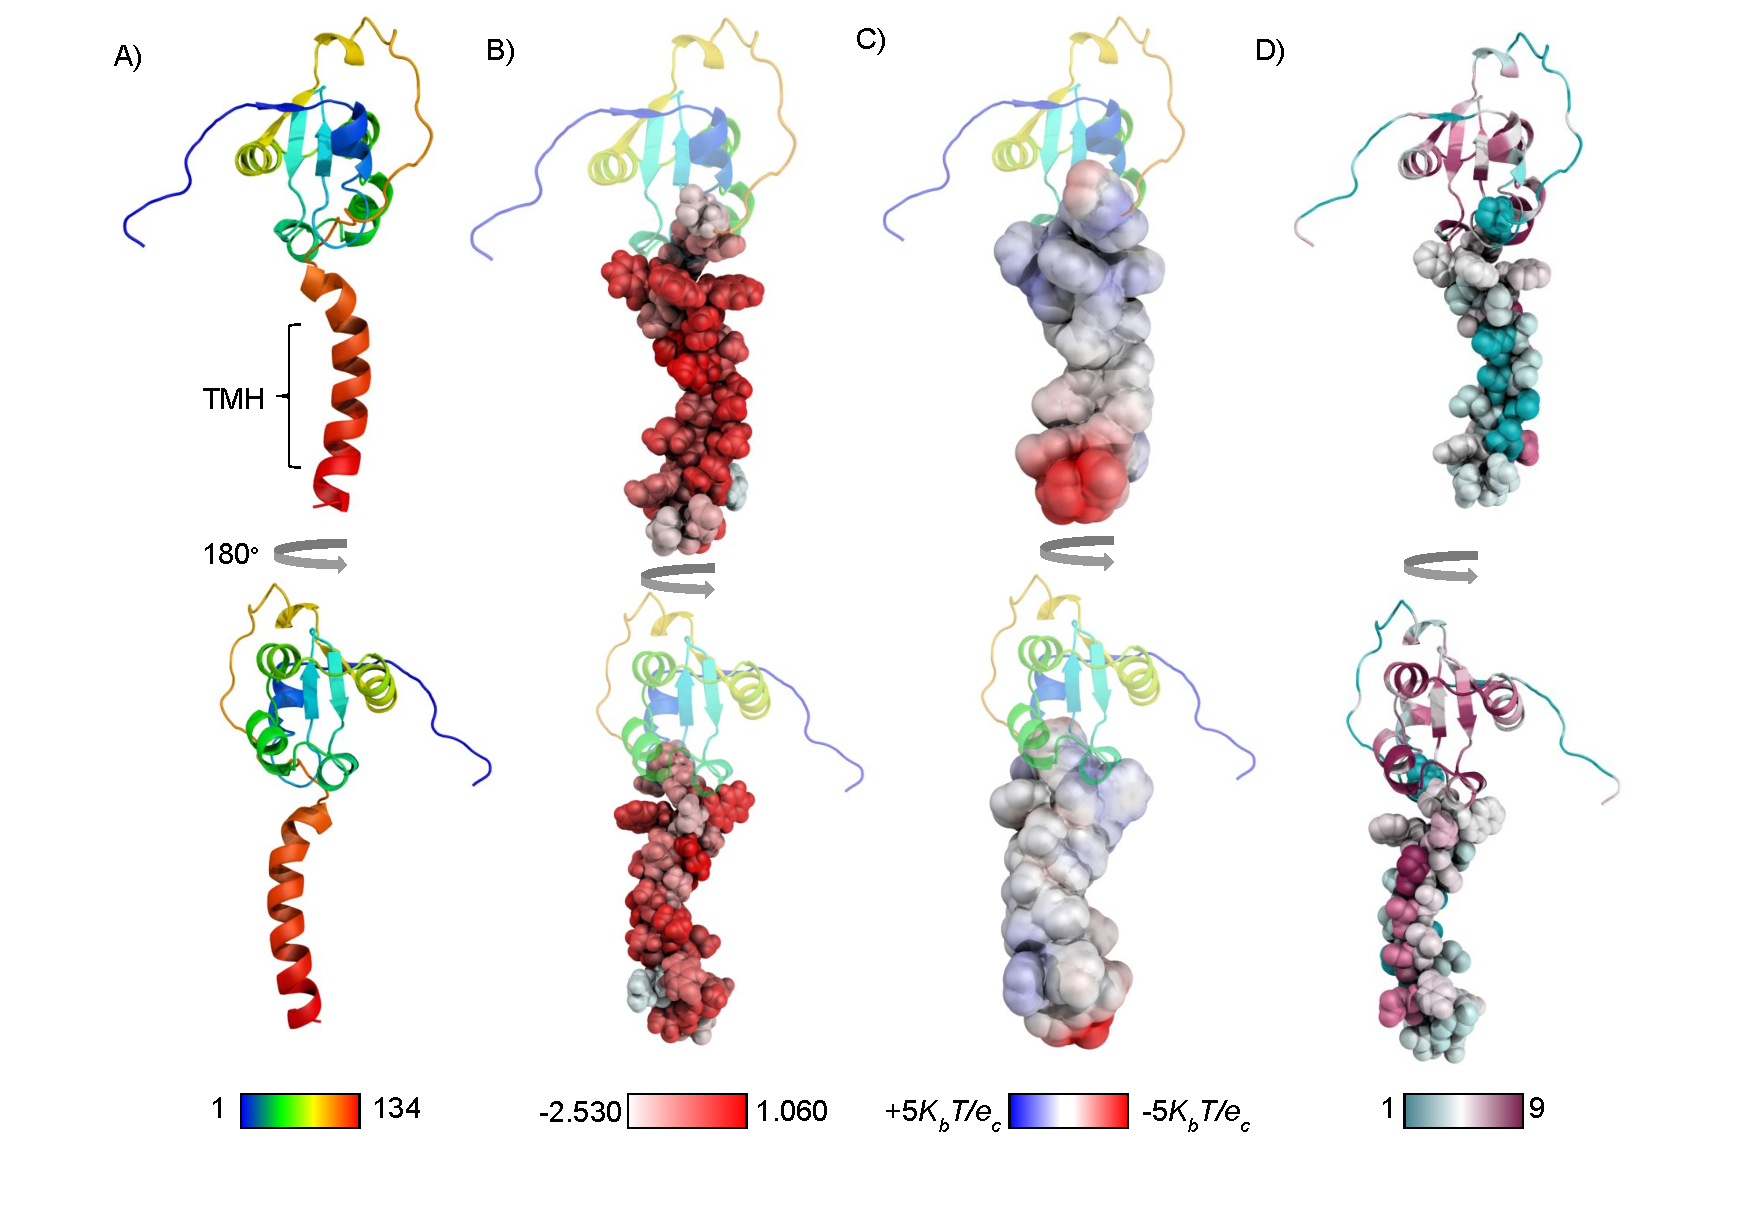
\includegraphics[width=1\textwidth]{TA_chapter/cytb5-biochemistry}
		\captionof{figure}[Structural biochemical analysis of a homology model of cytochrome b5.]{\textbf{Structural biochemical analysis of a homology model of cytochrome b5.}
		(A) The secondary structure of the protein coloured from the N terminus in blue to the C terminus in red coloured through the rainbow according to the residue number.
		(B) The hydrophobicity of the \gls{tmh} from white representing relatively polar residues to red showing relatively hydrophobic residues \cite{Eisenberg1984}.
		(C) The electrostatic surface with a threshold of $\pm5$ KT/e calculated by APBS in PyMol \cite{Baker2001}.
		Red patches are negatively charged whilst blue are positively charged.
		(D) The consurf scores on a scale of 1-9 (all residues had sufficient data) \cite{Ashkenazy2010}. Purple represents the the most conserved whilst blue is the least.
		Note the correlation between the highly and modestly conserved \gls{tmh} residues and the relatively polar residues.
		Another observable feature is the very strong ``positive inside'' \cite{VonHeijne1989, Andersson1992, Sharpe2010, Baeza-Delgado2013, Pogozheva2013} and ``negative outside'' features which are associated with anchorage \cite{Baker2017}.
}

\label{fig:cytb5-biochemistry}
\end{figure}

\section{Discussion}

We expect to see evolutionary adaptations of \gls{tmh} hydrophobicity to species specific membranes, even within eukaryotes~\cite{Baker2017, Sharpe2010}.
In this study using both a manually curated dataset from UniProt, and an automatically filtered list using SwissProt annotation, we do not observe any strong differences.
Why would we assume a stronger adaptation to organelles than to species?
Since we could not scrutinise a difference in the species, the strong hydrophobic differences between \gls{tmh}s from different organelles may not be solely accounted for by adaptation to the different membrane compositions.
Given the large biochemical distinction between \gls{ta} proteins with different terminal destinations, it is possible to conclude that \gls{tmh}s contain necessary, yet cryptic, biological factors that play a role in their targeting.
It is indeed possible that our observations are adaptations to the membrane environment, and this would not be unreasonable, except that \gls{ta} proteins would be expected to experience similar adaptations at a species level, for which at th  is sample size such an effect is unobservable.
This is almost certainly aided by other factors and is part of a system with several redundant mechanisms.

This could indeed be a cryptic functional similarity to the signal anchored proteins.
Signal anchored proteins contain a single hydrophobic segment that serves as both a mitochondrial targeting signal and a membrane anchor.
Interestingly, these proteins, along with some tail-anchored proteins, have been shown to be able to spontaneously insert into the membrane independently from the translocon~\cite{Elisa2012, Lan2000, Colombo2009}.

The idea that \gls{snare} proteins are modular and capable of spontaneous insertion has significant implications for both biomedical application in liposome-based drug delivery and can aid future research for testing complex biological molecular networks~\cite{Allen2013, Nordlund2014}.
